\documentclass[12pt,letterpaper]{article}
\usepackage[utf8]{inputenc}
\usepackage[spanish]{babel}
\usepackage{geometry}
\usepackage{fancyhdr}
\usepackage{graphicx}
\usepackage{xcolor}
\usepackage{amsmath}
\usepackage{parskip}
\usepackage{titlesec}
\usepackage{setspace}
\usepackage{float}
\usepackage{newtxtext,newtxmath}
\usepackage{array}
\usepackage{longtable}
\usepackage{hyperref}
\usepackage{tabularx}
\usepackage{caption}

\geometry{
    top=2.5cm,
    bottom=2.5cm,
    left=2.5cm,
    right=2.5cm,
    headheight=1.5cm,
    footskip=1cm
}

\titleformat{\section}{\large\bfseries}{\thesection.}{1em}{}
\titleformat{\subsection}{\normalsize\bfseries}{\thesubsection)}{1em}{}

\pagestyle{fancy}
\fancyhf{}
\fancyhead[L]{\small \textit{\nombreproyecto}}
\fancyhead[R]{\small \materia}
\fancyfoot[C]{\thepage}
\renewcommand{\headrulewidth}{0.4pt}

\newcommand{\universidad}{UNIVERSIDAD AUTÓNOMA DE SAN LUIS POTOSÍ}
\newcommand{\facultad}{Facultad de Ingeniería}
\newcommand{\carrera}{Ingeniería en Computación}
\newcommand{\materia}{Aplicaciones Web Escalables (224501)}
\newcommand{\nombreproyecto}{KitchenFlow: Control de Producción y Costeo para Cafeterías}
\newcommand{\autores}{Miguel Alejandro Gutiérrez Silva}
\newcommand{\fecha}{Semestre 2025-2026/II}
\newcommand{\profesor}{Ing. Francisco Javier Gómez Vázquez}

\newcommand{\ok}{\textbf{Implementado}}
\newcommand{\adj}{\textbf{Implementado con ajustes}}
\newcommand{\pend}{\textbf{No implementado}}

\begin{document}

\onecolumn
\singlespacing

\thispagestyle{empty}

\begin{center}
	\vspace*{0.5cm}

	{\color{black!70}\rule{\textwidth}{1.5pt}}

	\vspace{0.8cm}

	{\LARGE \textbf{\universidad}}

	\vspace{0.5cm}

	{\Large \facultad}

	\vspace{0.3cm}

	{\large \carrera}

	\vspace{0.8cm}

	{\color{black!40}\rule{0.6\textwidth}{0.5pt}}

	\vspace{0.8cm}

	{\large Documento de Entrega}

	\vspace{0.2cm}

	{\Large \textbf{\materia}}

	\vspace{1.5cm}

	\fbox{%
		\parbox{0.85\textwidth}{%
			\vspace{0.5cm}
			\centering
			{\LARGE \textbf{Reporte de Implementación}}

			\vspace{0.25cm}
			{\large \nombreproyecto}
			\vspace{0.5cm}
		}%
	}

	\vspace{1.5cm}

	\colorbox{black!5}{%
		\parbox{0.78\textwidth}{%
			\vspace{0.4cm}
			\begin{tabular}{rl}
				\textbf{Alumno:}   & \parbox[t]{8cm}{\autores} \\[0.6cm]
				\textbf{Profesor:} & \profesor                 \\[0.25cm]
				\textbf{Fecha:}    & \fecha                    \\
			\end{tabular}
			\vspace{0.4cm}
		}%
	}

	\vfill

	{\color{black!70}\rule{\textwidth}{1.5pt}}

	\vspace{0.3cm}

\end{center}

\newpage

\section{Propósito del documento}
Este documento resume el estado de implementación real de \textbf{KitchenFlow} con base en la propuesta obligatoria contenida en \texttt{report/propuesta/reporte\_template.tex}. El objetivo no es señalar cambios normales de diseño o de stack como defectos, sino distinguir con claridad entre:

\begin{itemize}
	\item funcionalidades que sí quedaron implementadas;
	\item funcionalidades que cambiaron de forma, pero conservan el objetivo de negocio;
	\item elementos que se ajustaron deliberadamente por razones prácticas de alcance o arquitectura.
\end{itemize}

\section{Resumen ejecutivo}
KitchenFlow evolucionó desde una propuesta visual a una aplicación funcional que ya cubre el flujo operativo principal de una cafetería:

\begin{center}
\textbf{abastecimiento \(\rightarrow\) recetas \(\rightarrow\) producción \(\rightarrow\) ventas \(\rightarrow\) dashboard}
\end{center}

Además, el sistema ya incluye autenticación basada en JWT, control de acceso por roles y una pantalla administrativa para gestión de usuarios. A nivel general, el proyecto \textbf{sí implementa el núcleo funcional planteado en la propuesta}. Las diferencias principales respecto al documento original se concentran en decisiones de arquitectura y en ajustes de experiencia de usuario, no en la ausencia del flujo central de negocio.

\section{Matriz de cobertura funcional}

\renewcommand{\arraystretch}{1.25}
\begin{longtable}{|p{3.5cm}|p{3.2cm}|p{2.4cm}|p{5.7cm}|}
\hline
\textbf{Elemento de la propuesta} & \textbf{Cobertura actual} & \textbf{Estado} & \textbf{Observación} \\
\hline
\endfirsthead

\hline
\textbf{Elemento de la propuesta} & \textbf{Cobertura actual} & \textbf{Estado} & \textbf{Observación} \\
\hline
\endhead

Autenticación JWT & Login, sesión actual, restauración de sesión y protección de API/webapp & \ok & Se implementó autenticación real basada en token y validación de sesión. \\
\hline
RBAC (Administrador, Cocina, Piso) & Roles predefinidos, guards frontend y middleware backend & \ok & El acceso está restringido por rol tanto en rutas Angular como en endpoints Express. \\
\hline
Gestión de usuarios por administrador & Alta, edición, activación/desactivación y restablecimiento de contraseña & \ok & Se agregó un módulo administrativo para completar este punto de la propuesta. \\
\hline
Recetario y costeo & CRUD de recetas, costo total, margen y estado de rentabilidad & \ok & El módulo ya funciona con datos reales y persiste costos calculados. \\
\hline
Costo Promedio Ponderado (WAC) & Registro de compras y recálculo inmediato de costo promedio por insumo & \ok & El flujo de abastecimiento actualiza stock y costo promedio ponderado. \\
\hline
Producción con explosión de materiales & Órdenes con estados, reserva de insumos, cierre con consumo real y merma por lote & \ok & La producción ya no es mockup; es una operación con control de inventario y resultados reales. \\
\hline
Control de mermas & Merma integrada en el cierre de producción mediante consumo real vs. planeado y resumen de desperdicio & \adj & No existe como módulo independiente, pero la información requerida sí se registra y se usa en analítica. \\
\hline
Despacho / ventas en piso & Registro real de ventas, decremento de stock terminado y ticket persistido & \ok & El personal de piso puede operar sobre producto terminado disponible. \\
\hline
Dashboard de rentabilidad & Indicadores reales de ventas, producción, compras, alertas y productos críticos & \ok & El dashboard consume datos reales del backend, no datos mockeados. \\
\hline
Mockups principales & Dashboard, recetas, producción, ventas y abastecimiento reimplementados como pantallas funcionales & \ok & Las pantallas propuestas ya están representadas como módulos operativos. \\
\hline
Conversión de unidades & Catálogo uniforme de unidades, sin motor genérico de conversión entre unidades heterogéneas & \adj & Se normalizó la captura de unidades para evitar complejidad adicional innecesaria en el alcance actual. \\
\hline
Auditoría operativa de producción & Historial por orden con estados, tiempos, cantidades reales y costos de merma & \ok & El flujo de producción conserva trazabilidad suficiente para revisión posterior. \\
\hline
\end{longtable}

\section{Cambios entre propuesta e implementación}

La tabla siguiente resume \textbf{qué cambió}, \textbf{qué se implementó realmente} y \textbf{por qué ese cambio fue razonable dentro del desarrollo del proyecto}.

\renewcommand{\arraystretch}{1.25}
\begin{longtable}{|p{3.2cm}|p{3.8cm}|p{3.8cm}|p{4.2cm}|}
\hline
\textbf{Tema} & \textbf{Propuesta original} & \textbf{Implementación final} & \textbf{Motivo del ajuste} \\
\hline
\endfirsthead

\hline
\textbf{Tema} & \textbf{Propuesta original} & \textbf{Implementación final} & \textbf{Motivo del ajuste} \\
\hline
\endhead

Stack backend & Hono + ZenStack/Prisma + PostgreSQL 16 & Express + Mongoose + MongoDB & Se decidió consolidar la implementación sobre el stack realmente utilizado por el proyecto y por el entorno de despliegue. El cambio es de arquitectura, no de objetivo funcional. \\
\hline
Contratos compartidos & RPC/DTOs derivados de Zod & OpenAPI + cliente tipado generado para Angular & Se mantuvo la idea de contrato tipado compartido, pero usando OpenAPI como mecanismo más compatible con el stack real. \\
\hline
Abastecimiento & Wizard de 4 pasos & Tabla operativa de insumos + modales de compra e historial & Se privilegió una interacción más útil para uso real diario, manteniendo el propósito del módulo. \\
\hline
Recetas & Editor de receta tipo maestro-detalle & Editor modal con costeo, margen y persistencia real & Se conservó el objetivo del mockup, pero con una UI ajustada al patrón final del sistema. \\
\hline
Producción & Registro atómico simple de lote & Órdenes con estados, apartados, cierre real y merma asociada & El modelo evolucionó para reflejar mejor la operación real de cocina y el control de recursos. \\
\hline
Mermas & Módulo explícito en propuesta & Información absorbida en cierre de producción y dashboard & Para el alcance final, la merma quedó integrada al flujo donde realmente se origina la desviación. \\
\hline
Ventas & Mockup tipo terminal táctil & Tabla de productos vendibles + modal de ticket y ventas recientes & Se simplificó la interacción sin perder el despacho inmediato de producto terminado. \\
\hline
Dashboard & KPIs y comparativas mensuales & KPIs reales, tendencias, alertas, productos críticos y actividad reciente & Se priorizó mostrar información accionable basada en datos ya disponibles del sistema. \\
\hline
Usuarios & Gestión administrativa implícita en el rol ADMIN & Pantalla específica de gestión de usuarios & Se agregó para cerrar una ausencia funcional importante respecto a la propuesta. \\
\hline
Conversión de unidades & Conversión explícita entre unidad de compra y unidad de consumo & Catálogo uniforme de unidades capturadas de forma operativa & Se acotó el problema usando normalización desde la captura, suficiente para el alcance académico implementado. \\
\hline
\end{longtable}

\section{Arquitectura implementada}
La arquitectura final de KitchenFlow se consolidó como una solución desacoplada de dos capas principales:

\begin{itemize}
	\item \textbf{Frontend Angular 21}: interfaz de usuario con rutas lazy, guards por rol, cliente tipado generado desde OpenAPI y componentes standalone bajo un sistema visual local inspirado en ZardUI.
	\item \textbf{Backend Express + MongoDB}: API REST con autenticación JWT, middleware de autorización por rol, lógica de negocio para inventario, recetas, producción, ventas, usuarios y analítica.
\end{itemize}

Aunque la propuesta original planteaba Hono, ZenStack, Prisma y PostgreSQL, la implementación real se estabilizó sobre \textbf{Express + Mongoose + MongoDB}. Este cambio permitió trabajar sobre el stack que efectivamente estaba en uso dentro del repositorio, reduciendo fricción de integración y conservando el objetivo principal de la propuesta: un sistema funcional, tipado y desplegable.

En términos de intercambio de datos, la integridad entre frontend y backend se resolvió mediante:
\begin{itemize}
	\item \textbf{OpenAPI} como contrato formal de la API;
	\item \textbf{generación de tipos} para Angular a partir del esquema OpenAPI;
	\item \textbf{validación operativa por capas} a través de controladores, modelos y middleware del backend.
\end{itemize}

Esta arquitectura implementada mantiene el espíritu de la propuesta original al conservar separación de responsabilidades, tipado entre capas y control explícito del dominio de negocio.

\begin{figure}[!htbp]
	\centering
	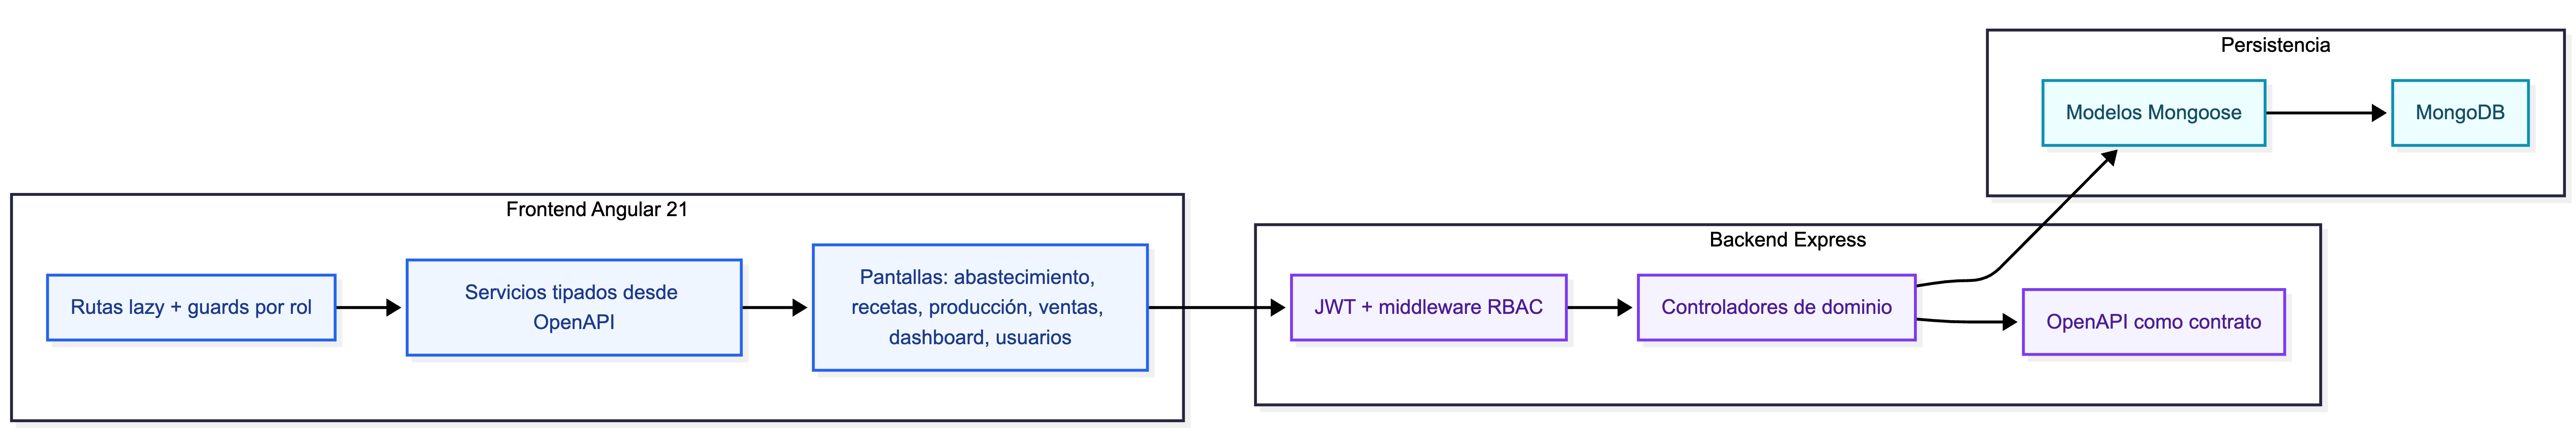
\includegraphics[width=\textwidth,height=0.31\textheight,keepaspectratio]{diagramas/arquitectura_implementada.png}
	\caption{Arquitectura implementada de KitchenFlow.}
\end{figure}

\section{Dockerización}
El proyecto fue preparado para ejecutarse de forma consistente mediante contenedores Docker coordinados por \texttt{docker-compose.yml}. La composición actual contempla tres servicios:

\begin{itemize}
	\item \textbf{frontend}: aplicación Angular servida en desarrollo con hot reload;
	\item \textbf{backend}: API Express con reinicio automático durante desarrollo;
	\item \textbf{mongo}: instancia de MongoDB para persistencia del sistema.
\end{itemize}

Esta decisión aporta varias ventajas prácticas:
\begin{itemize}
	\item unifica el entorno de desarrollo entre máquinas;
	\item reduce diferencias entre entorno local y entorno desplegado;
	\item simplifica el arranque del proyecto completo;
	\item facilita la futura reproducción o evaluación del sistema.
\end{itemize}

Además, la aplicación fue configurada para que el frontend consuma la API bajo la misma solución desplegada, conservando una estructura clara de puertos y servicios. En términos académicos y operativos, la dockerización permitió demostrar no sólo la lógica del sistema, sino también su \textbf{capacidad real de puesta en marcha}.

\begin{figure}[!htbp]
	\centering
	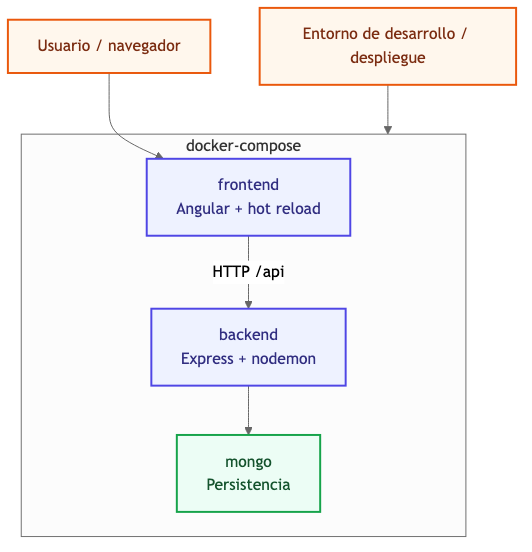
\includegraphics[width=0.82\textwidth,height=0.29\textheight,keepaspectratio]{diagramas/dockerizacion.png}
	\caption{Esquema de dockerización usado en el proyecto.}
\end{figure}

\section{CI/CD y despliegue}
El proyecto también incorpora una estrategia de integración y despliegue continuo alineada con la implementación final. Se configuró un flujo de despliegue utilizando \textbf{GitHub Actions} con un \textbf{runner self-hosted} que se ejecuta en un \textbf{VPS propio}.

Esto implica que:
\begin{itemize}
	\item el repositorio puede disparar procesos automáticos de despliegue;
	\item el runner no depende de infraestructura efímera externa;
	\item la construcción y levantamiento del sistema ocurren directamente sobre el servidor de destino.
\end{itemize}

En términos prácticos, el pipeline permite:
\begin{itemize}
	\item obtener el código más reciente del repositorio;
	\item reconstruir los servicios necesarios;
	\item levantar el sistema mediante Docker Compose;
	\item verificar la disponibilidad básica del frontend y del backend.
\end{itemize}

El hecho de contar con un \textbf{VPS propio que también hospeda el runner} fortalece el carácter de entrega del proyecto, ya que no se trata únicamente de una implementación local o académica, sino de una solución que fue preparada para correr en infraestructura controlada por el autor.

\begin{figure}[!htbp]
	\centering
	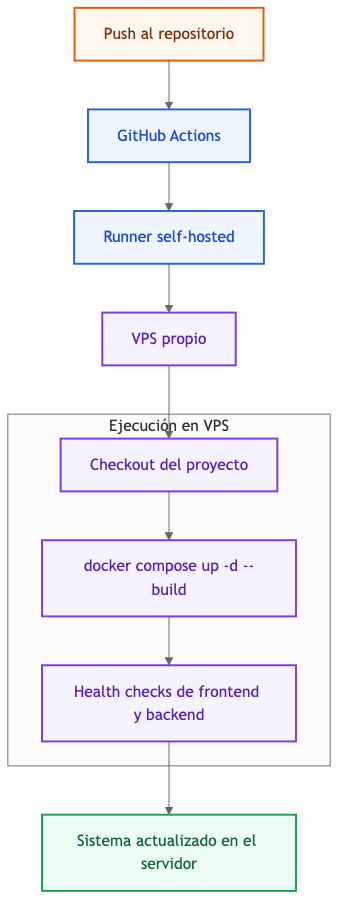
\includegraphics[width=0.9\textwidth,height=0.36\textheight,keepaspectratio]{diagramas/cicd_vps.png}
	\caption{Flujo de CI/CD con runner self-hosted ejecutándose en VPS propio.}
\end{figure}

\section{Capturas del sistema}
Como evidencia complementaria de la implementación, se incluyen a continuación capturas reales de la interfaz operativa de KitchenFlow. Las imágenes fueron generadas directamente sobre la aplicación en ejecución y muestran el estado actual de los módulos principales.

\begin{figure}[!htbp]
	\centering
	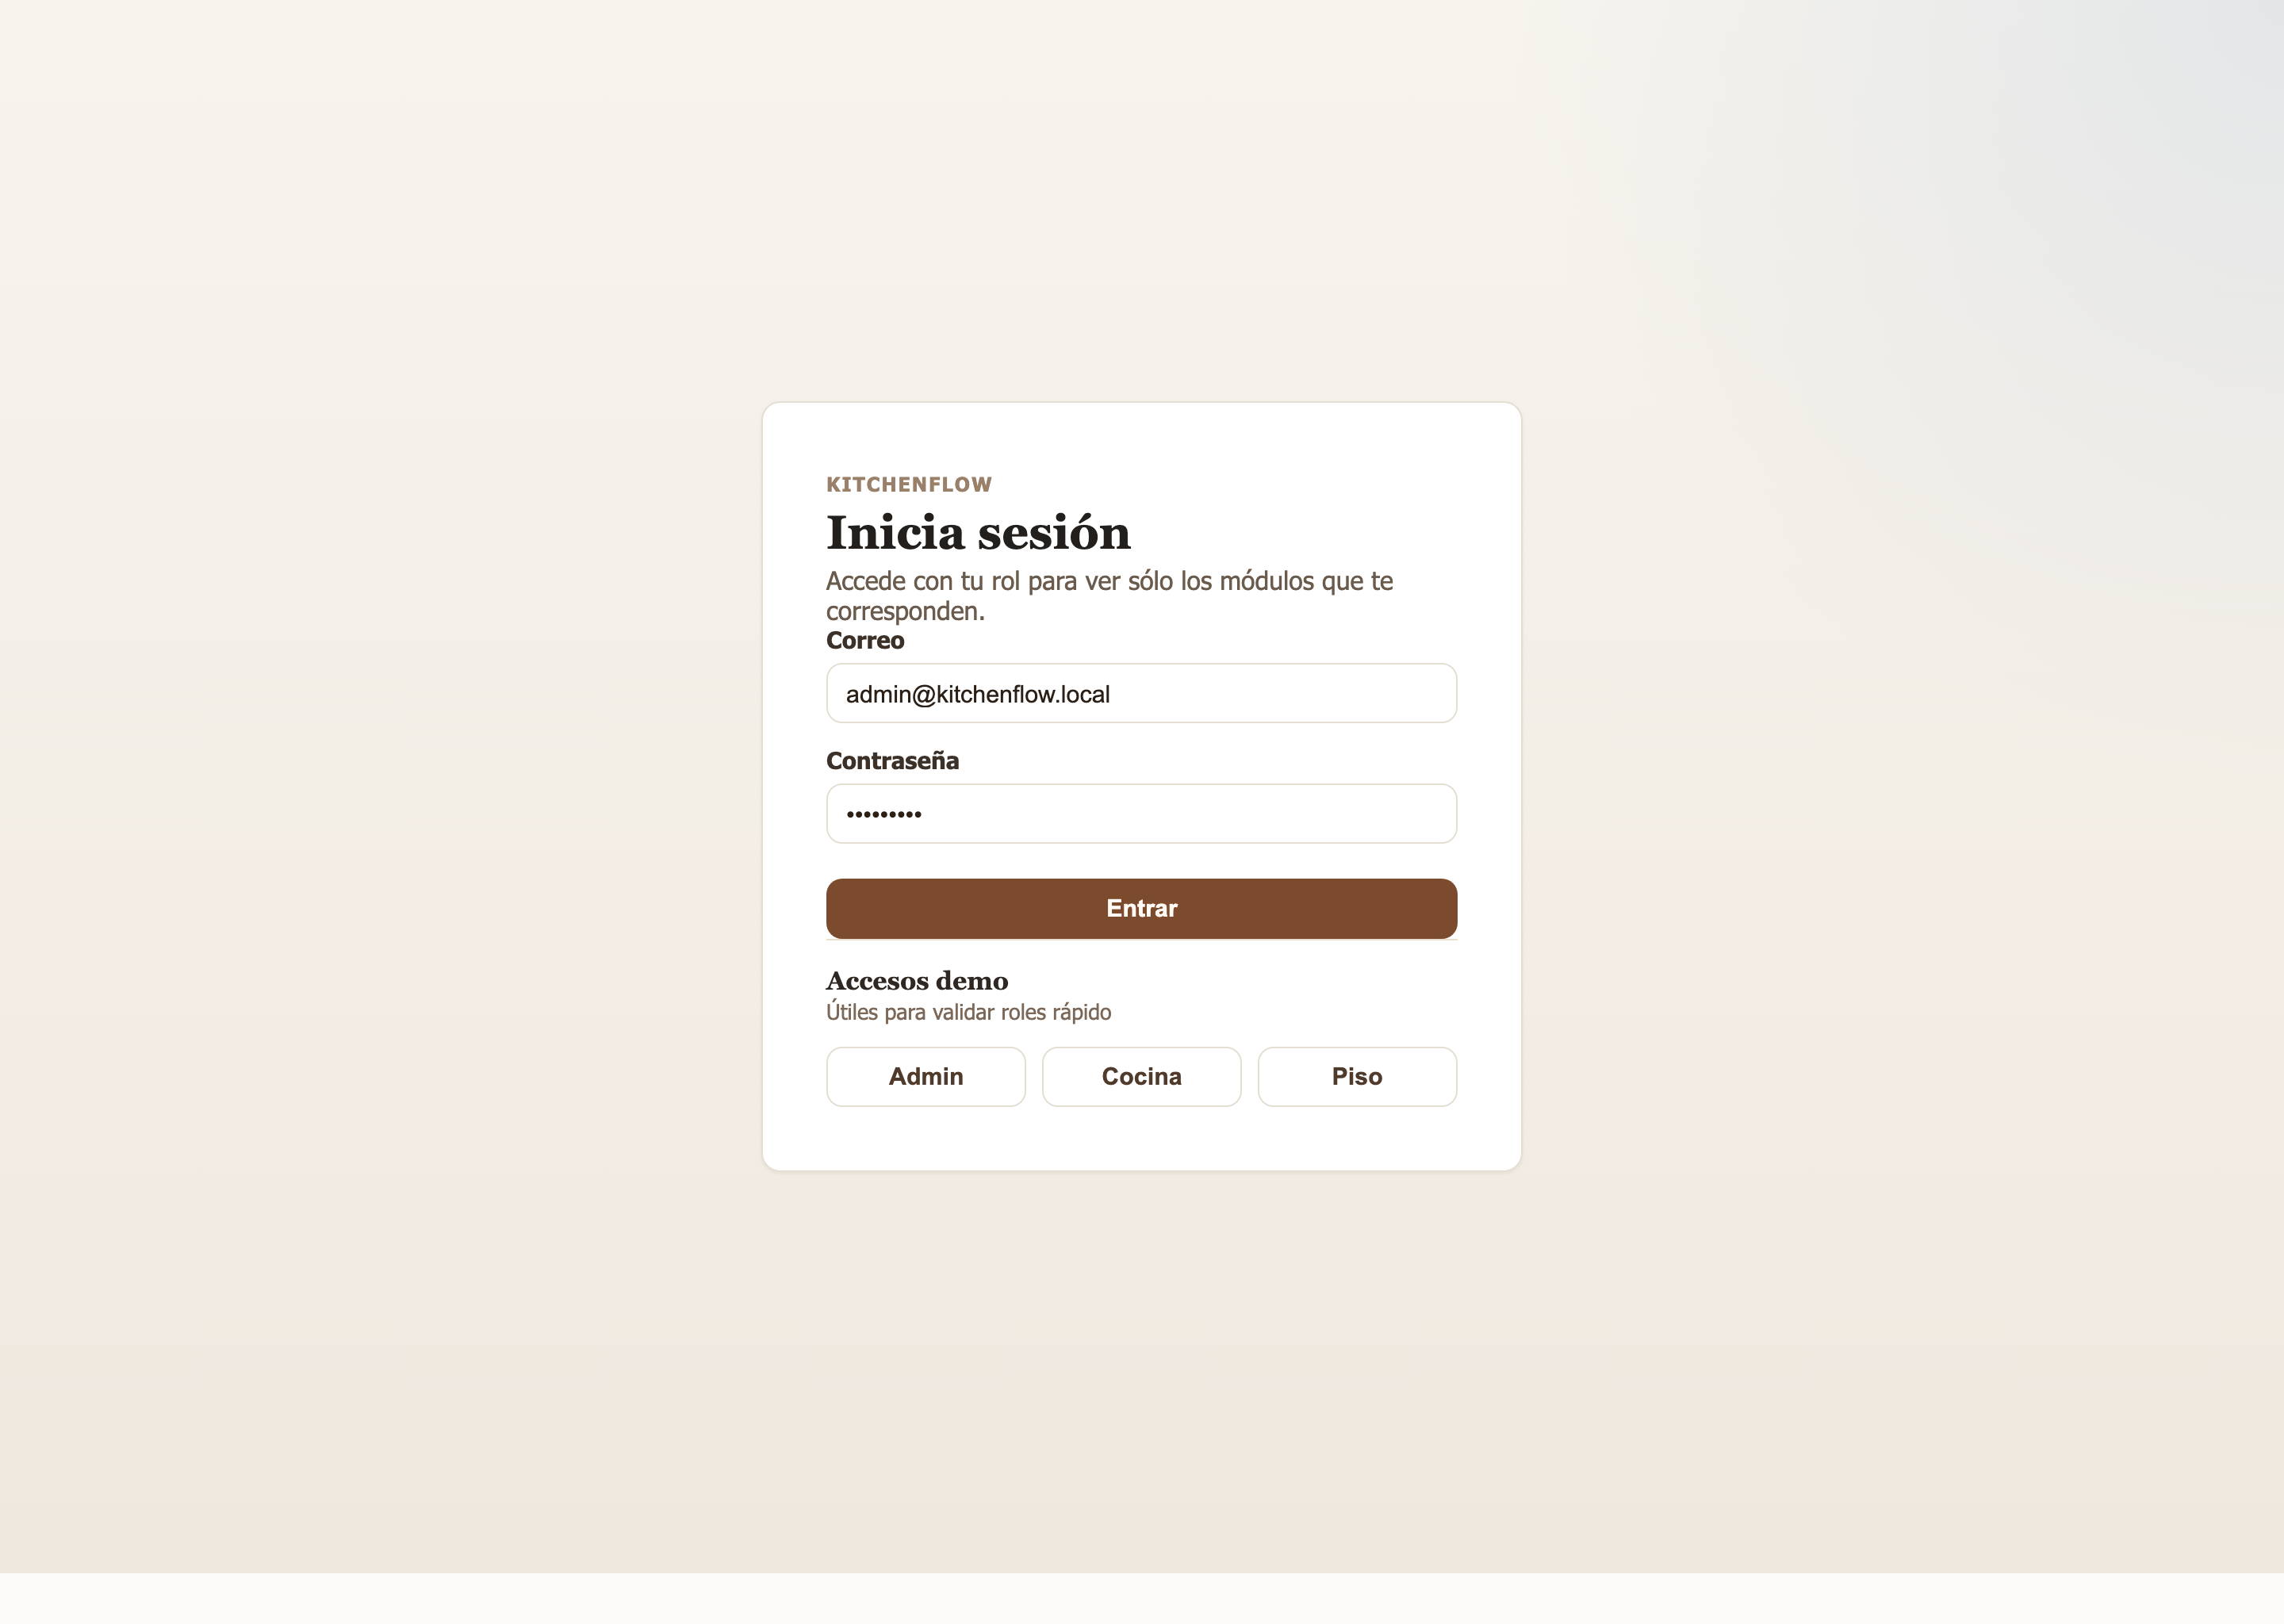
\includegraphics[width=0.86\textwidth,height=0.34\textheight,keepaspectratio]{capturas/login.png}
	\caption{Pantalla de inicio de sesión de KitchenFlow. Se muestran accesos diferenciados por rol para administrador, cocina y piso de ventas.}
\end{figure}

\begin{figure}[!htbp]
	\centering
	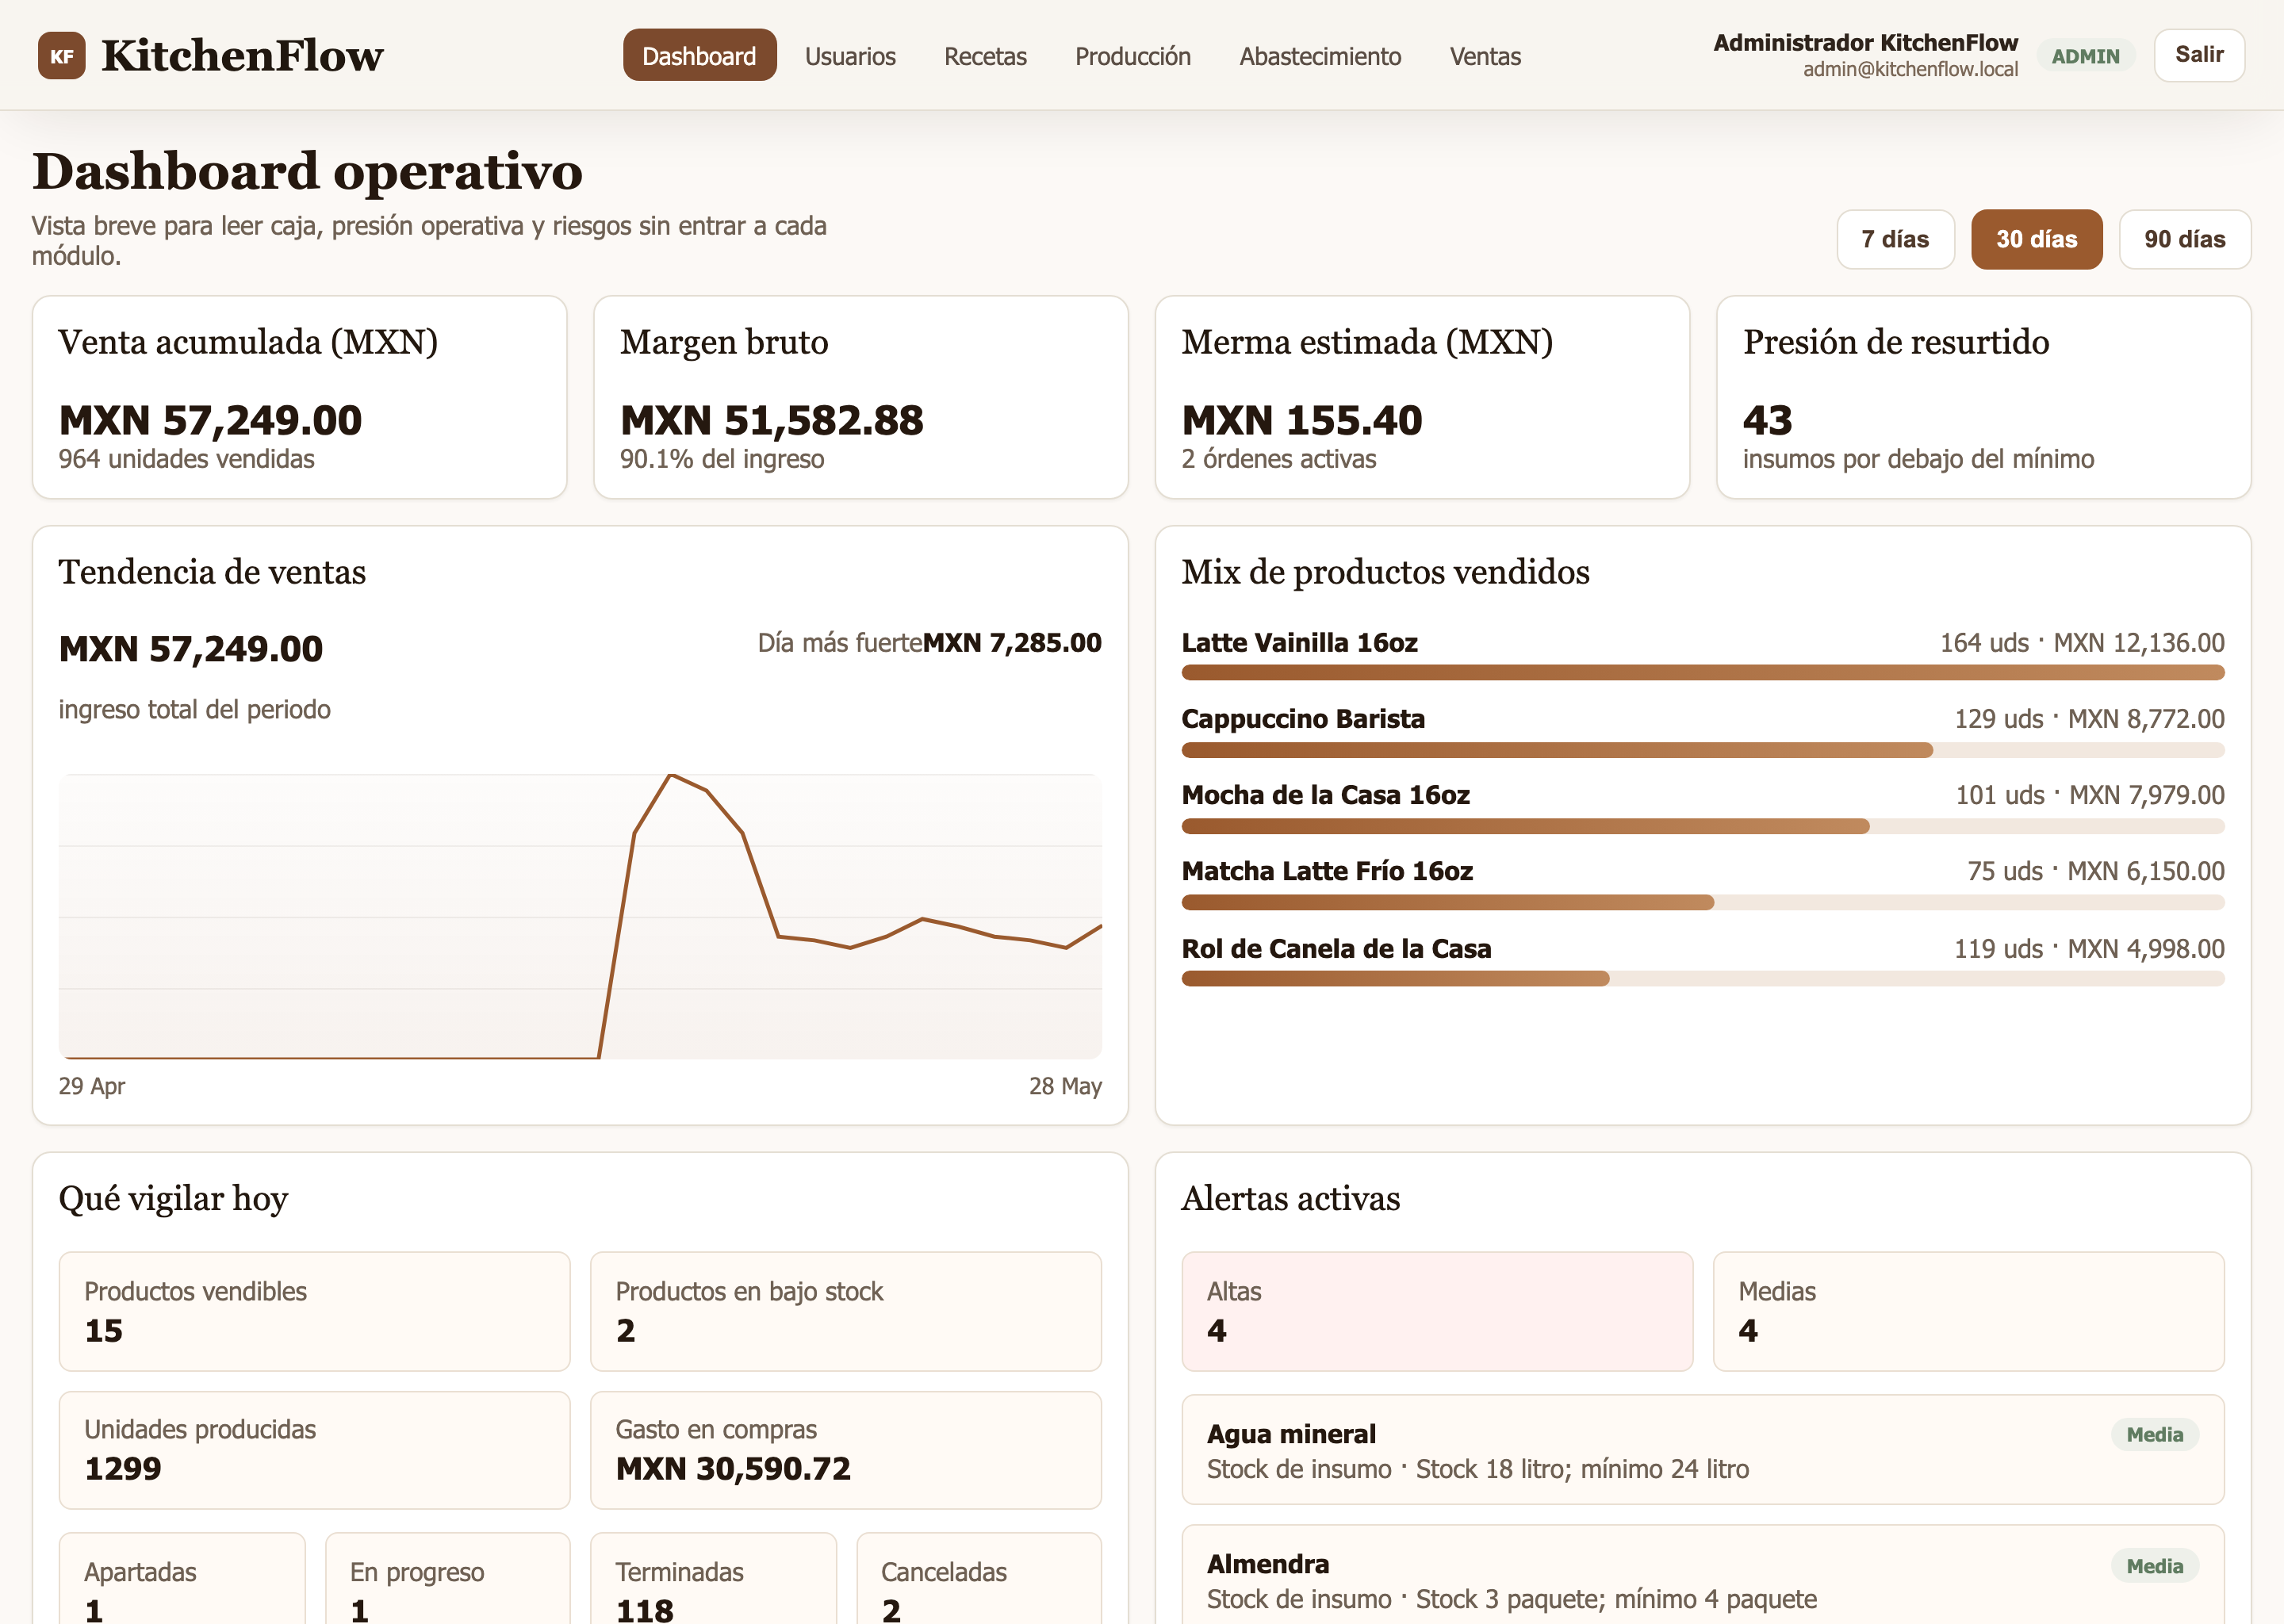
\includegraphics[width=0.92\textwidth,height=0.34\textheight,keepaspectratio]{capturas/dashboard.png}
	\caption{Dashboard operativo con indicadores reales de ventas, margen, merma, resurtido, tendencias y alertas de operación.}
\end{figure}

\begin{figure}[!htbp]
	\centering
	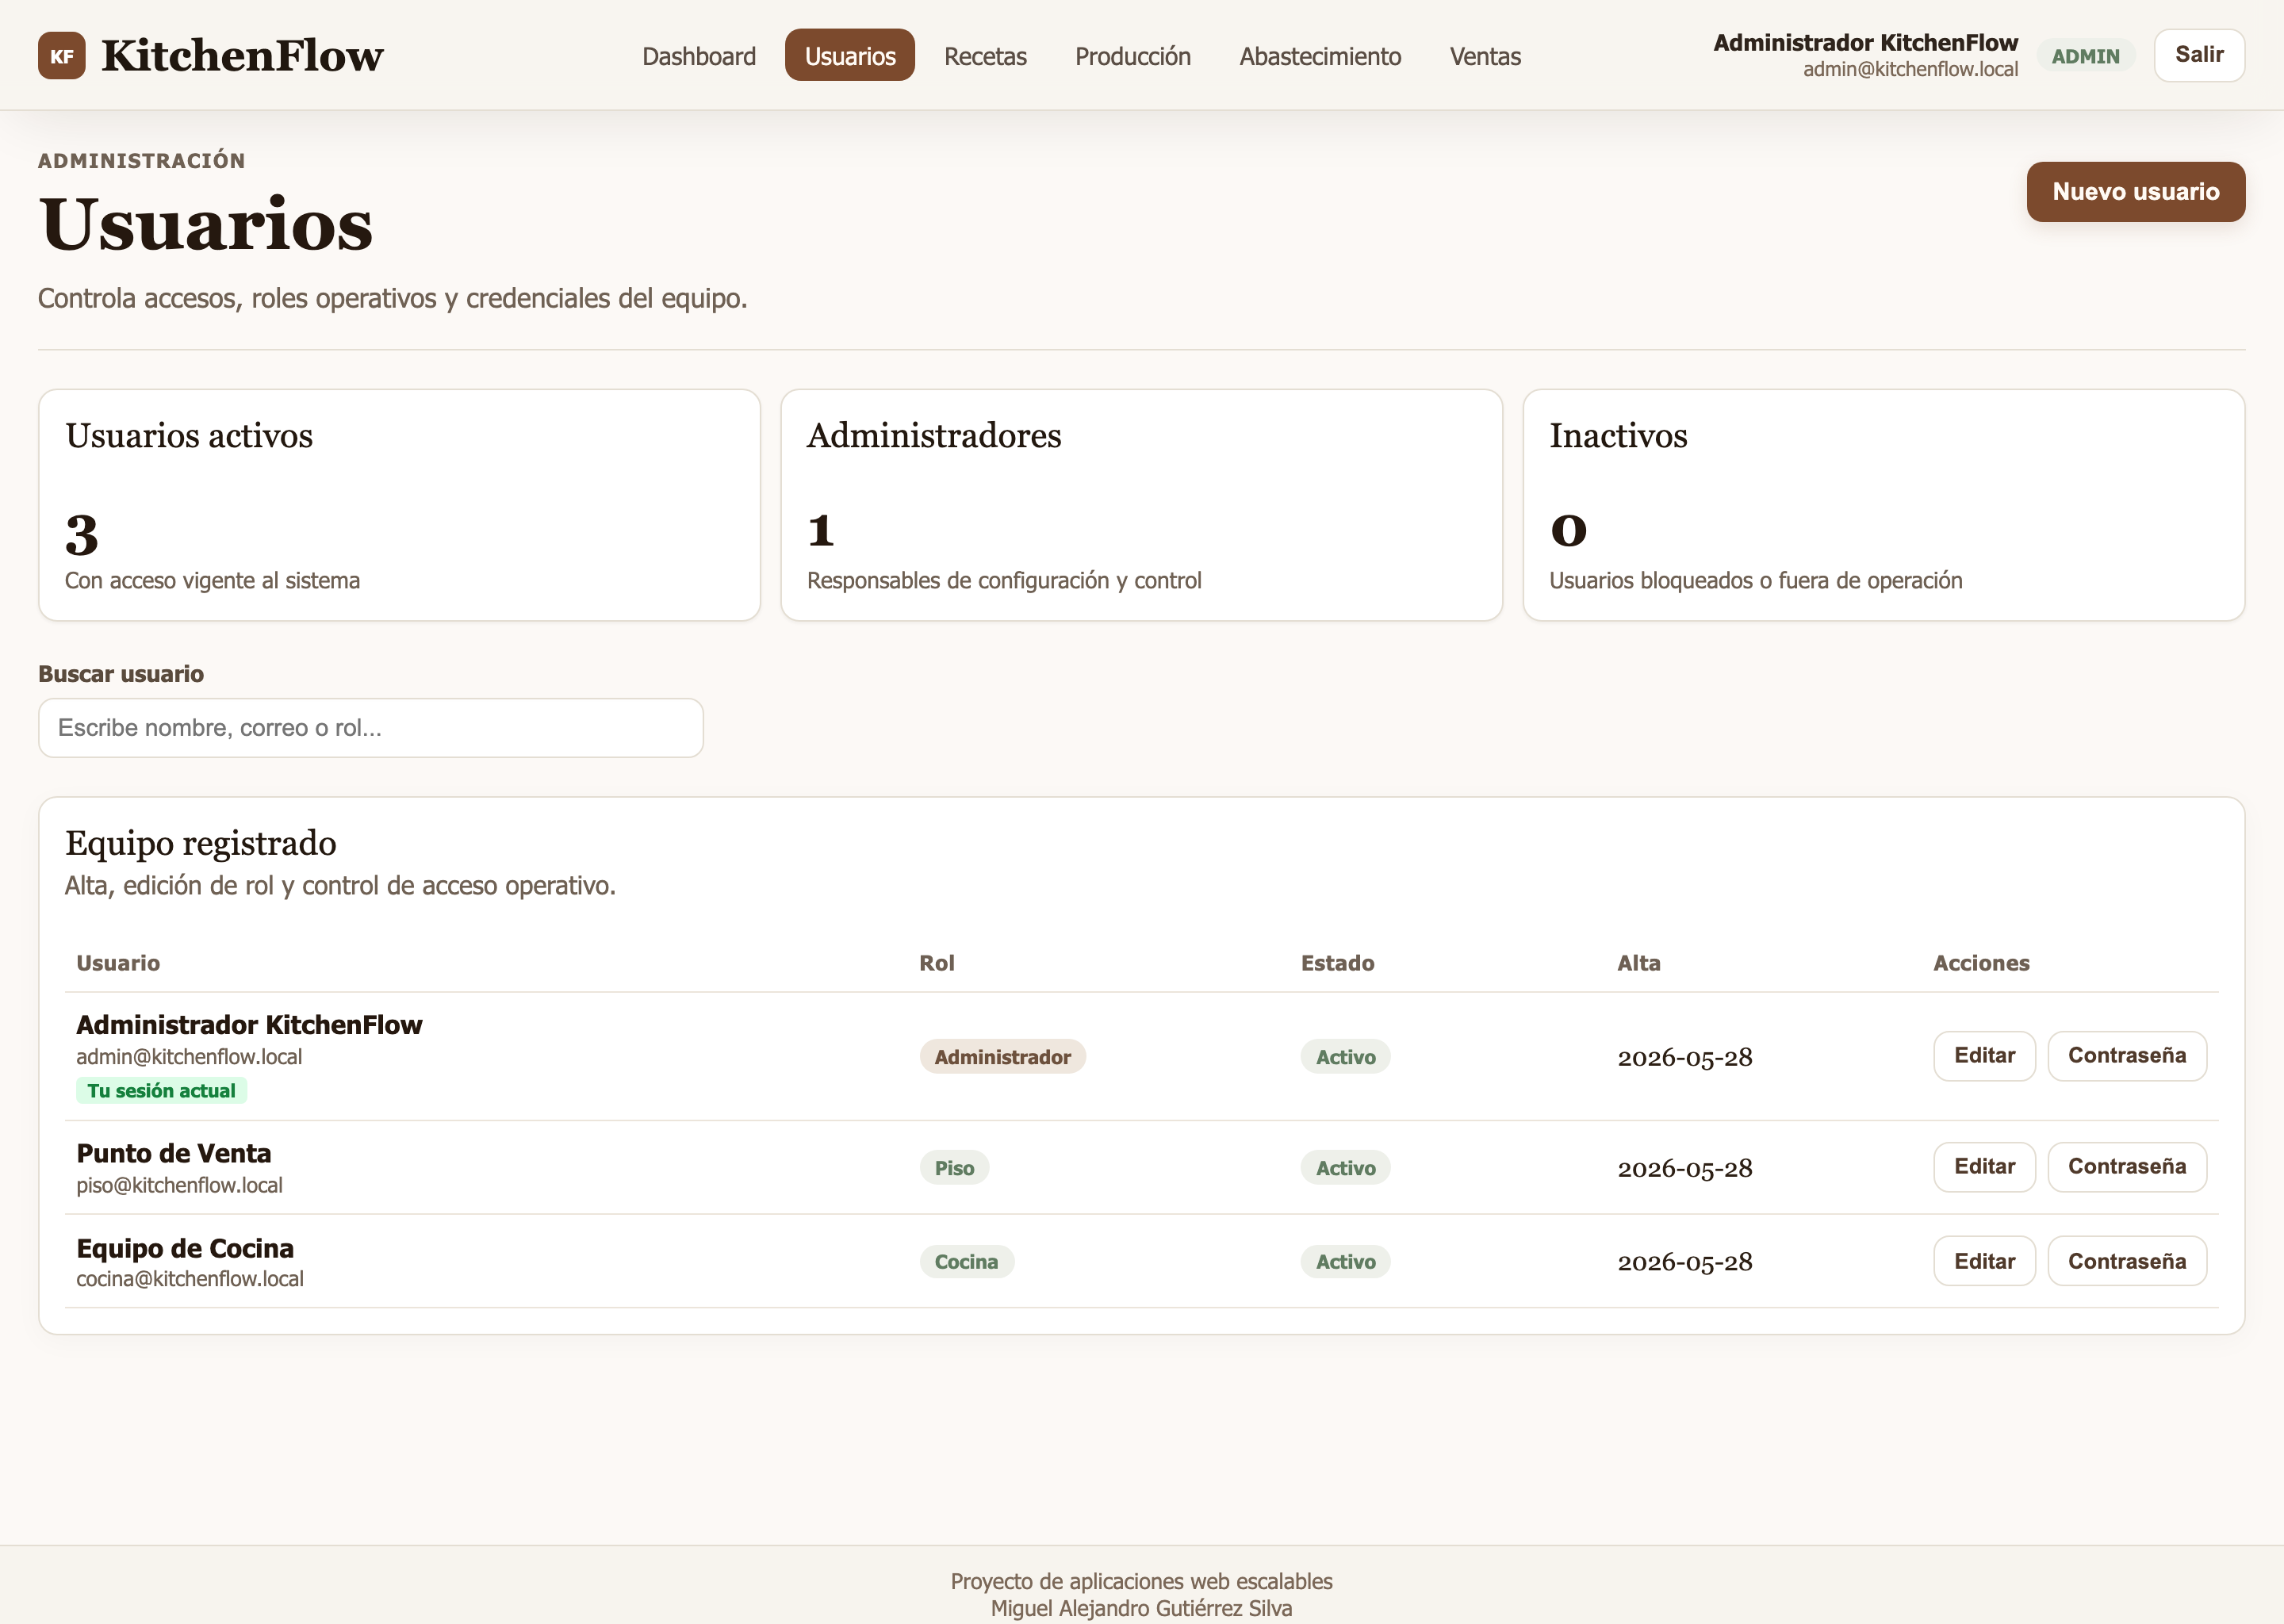
\includegraphics[width=0.92\textwidth,height=0.34\textheight,keepaspectratio]{capturas/usuarios.png}
	\caption{Módulo de gestión de usuarios. El administrador puede consultar cuentas activas, altas recientes, roles y acciones de mantenimiento.}
\end{figure}

\begin{figure}[!htbp]
	\centering
	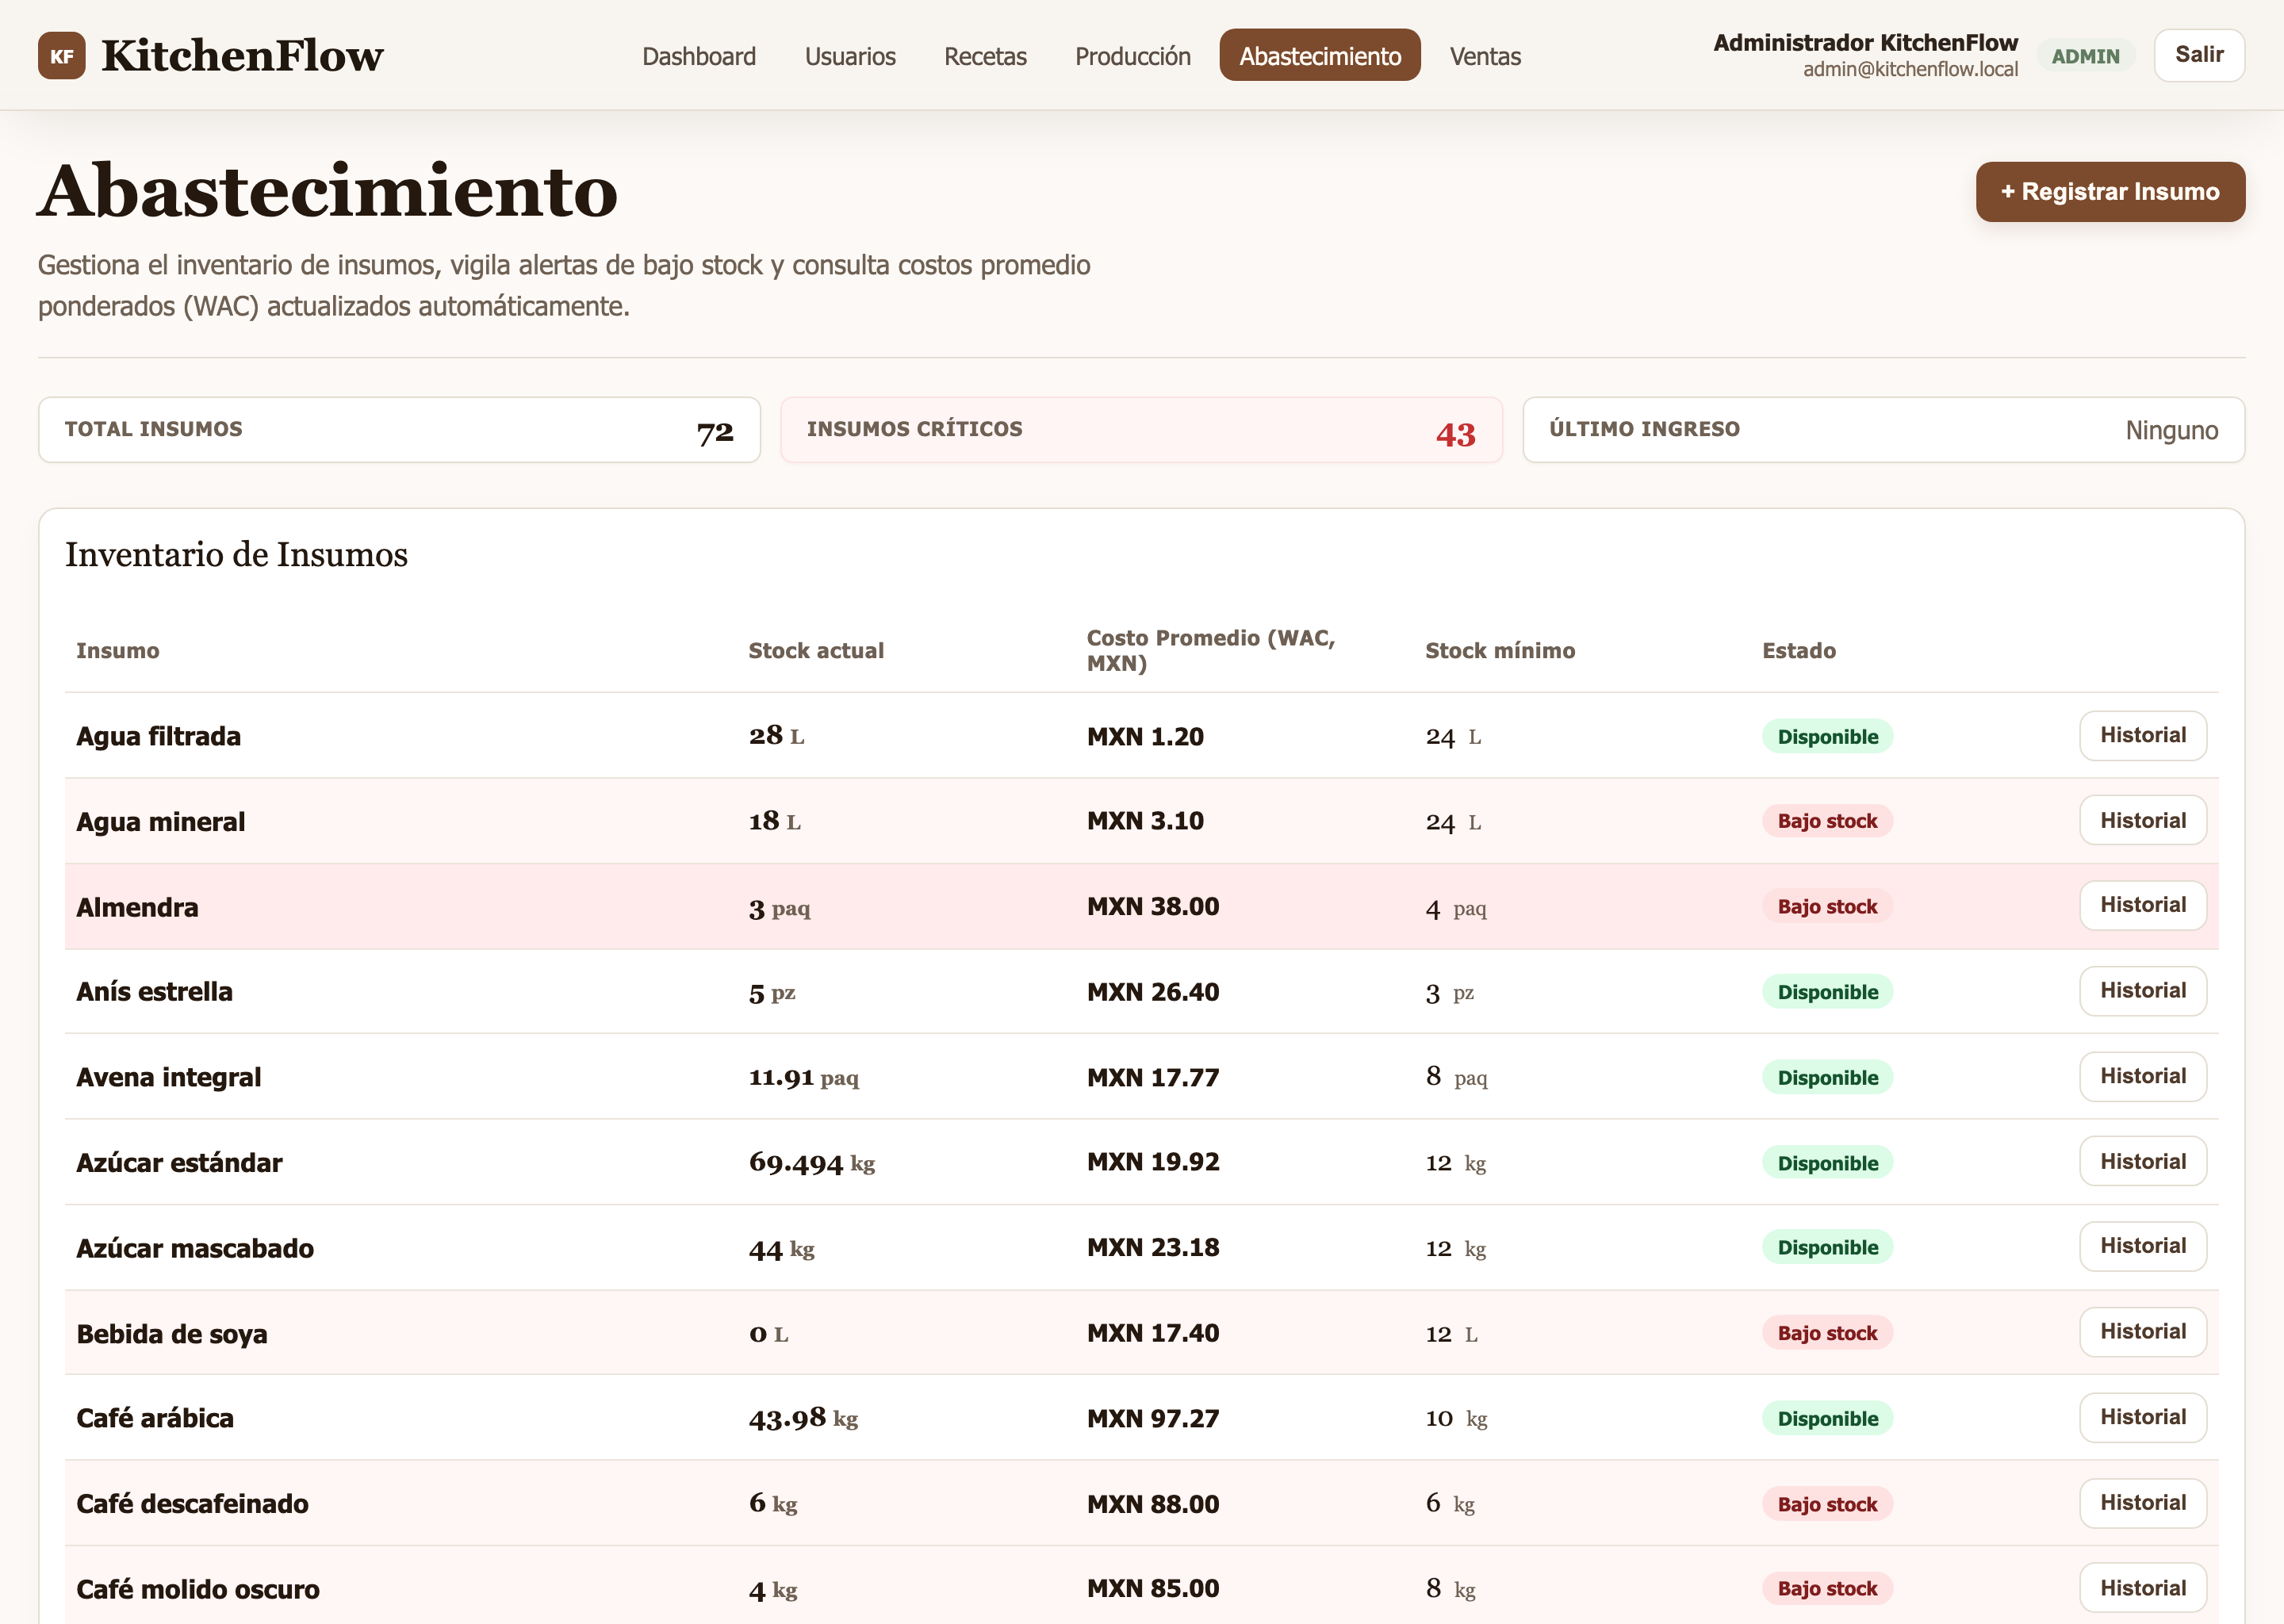
\includegraphics[width=0.92\textwidth,height=0.34\textheight,keepaspectratio]{capturas/abastecimiento.png}
	\caption{Módulo de abastecimiento con inventario de insumos, costo promedio ponderado, stock mínimo y control de historial de compras.}
\end{figure}

\begin{figure}[!htbp]
	\centering
	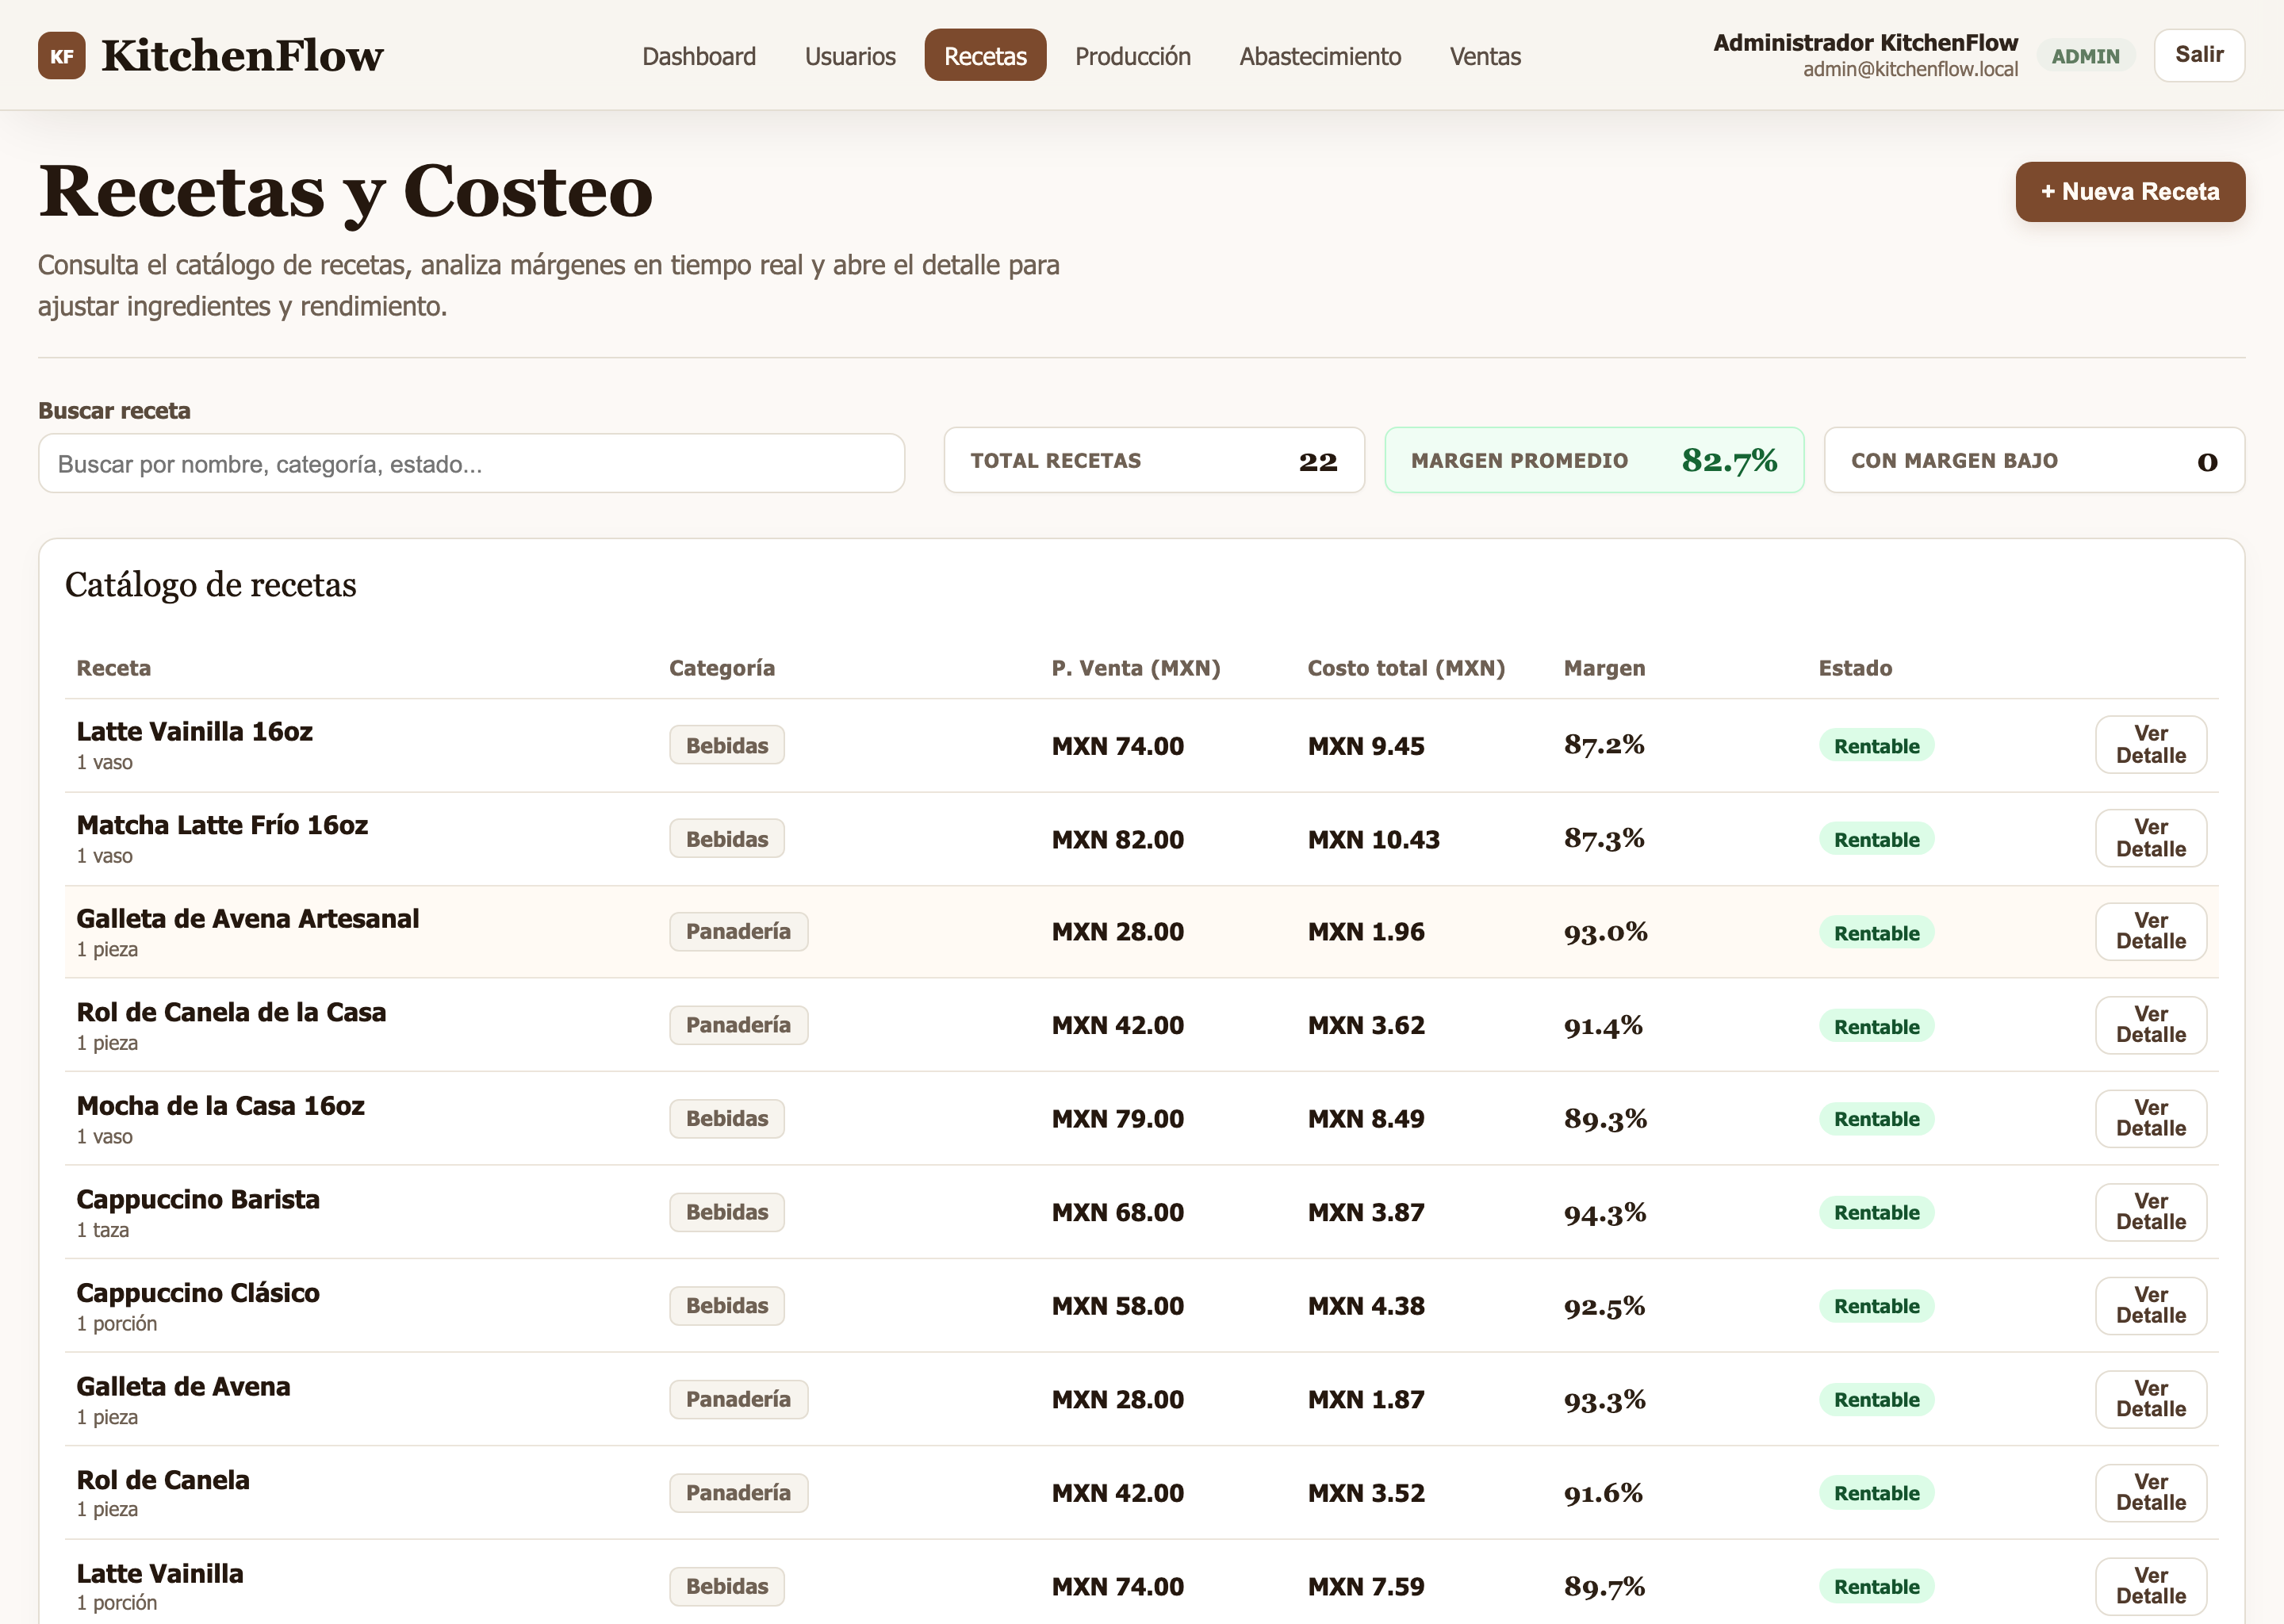
\includegraphics[width=0.92\textwidth,height=0.34\textheight,keepaspectratio]{capturas/recetas.png}
	\caption{Pantalla de recetas y costeo. Se muestran catálogo, costos unitarios, precio de venta, margen y estado de rentabilidad por producto.}
\end{figure}

\begin{figure}[!htbp]
	\centering
	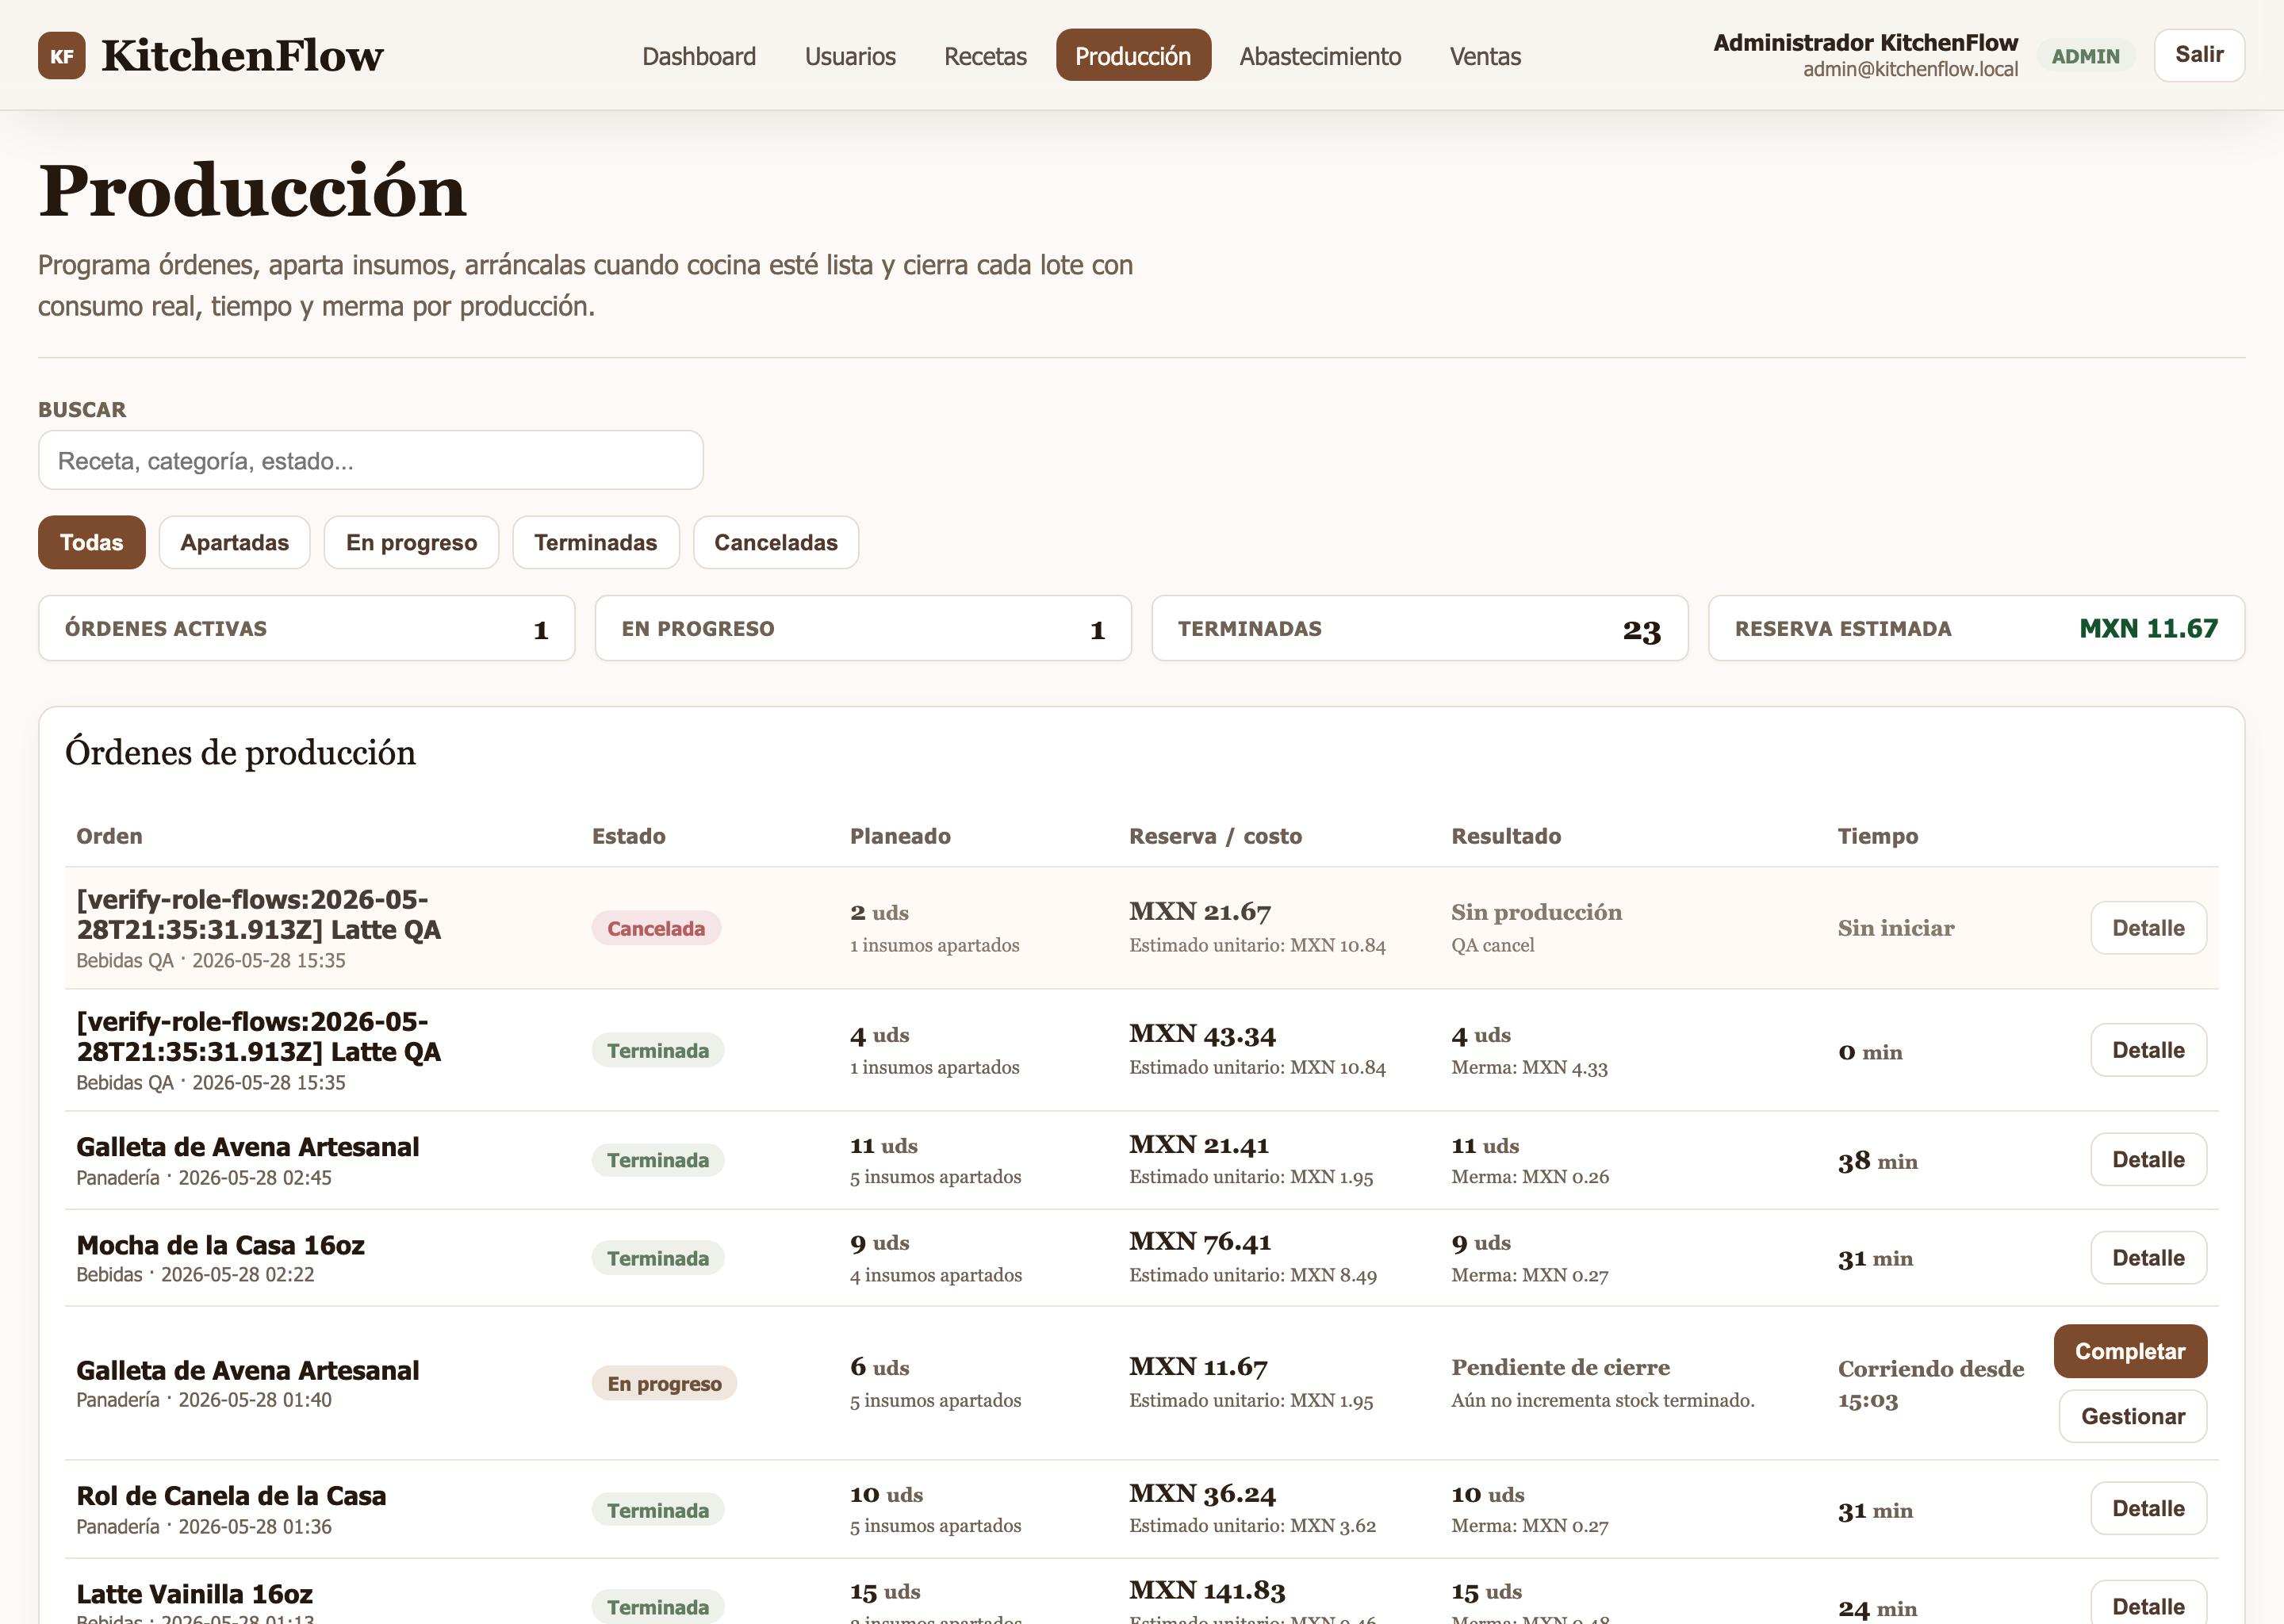
\includegraphics[width=0.92\textwidth,height=0.34\textheight,keepaspectratio]{capturas/produccion.png}
	\caption{Módulo de producción con órdenes por estado, costos planeados, resultados reales y seguimiento operativo del lote.}
\end{figure}

\begin{figure}[!htbp]
	\centering
	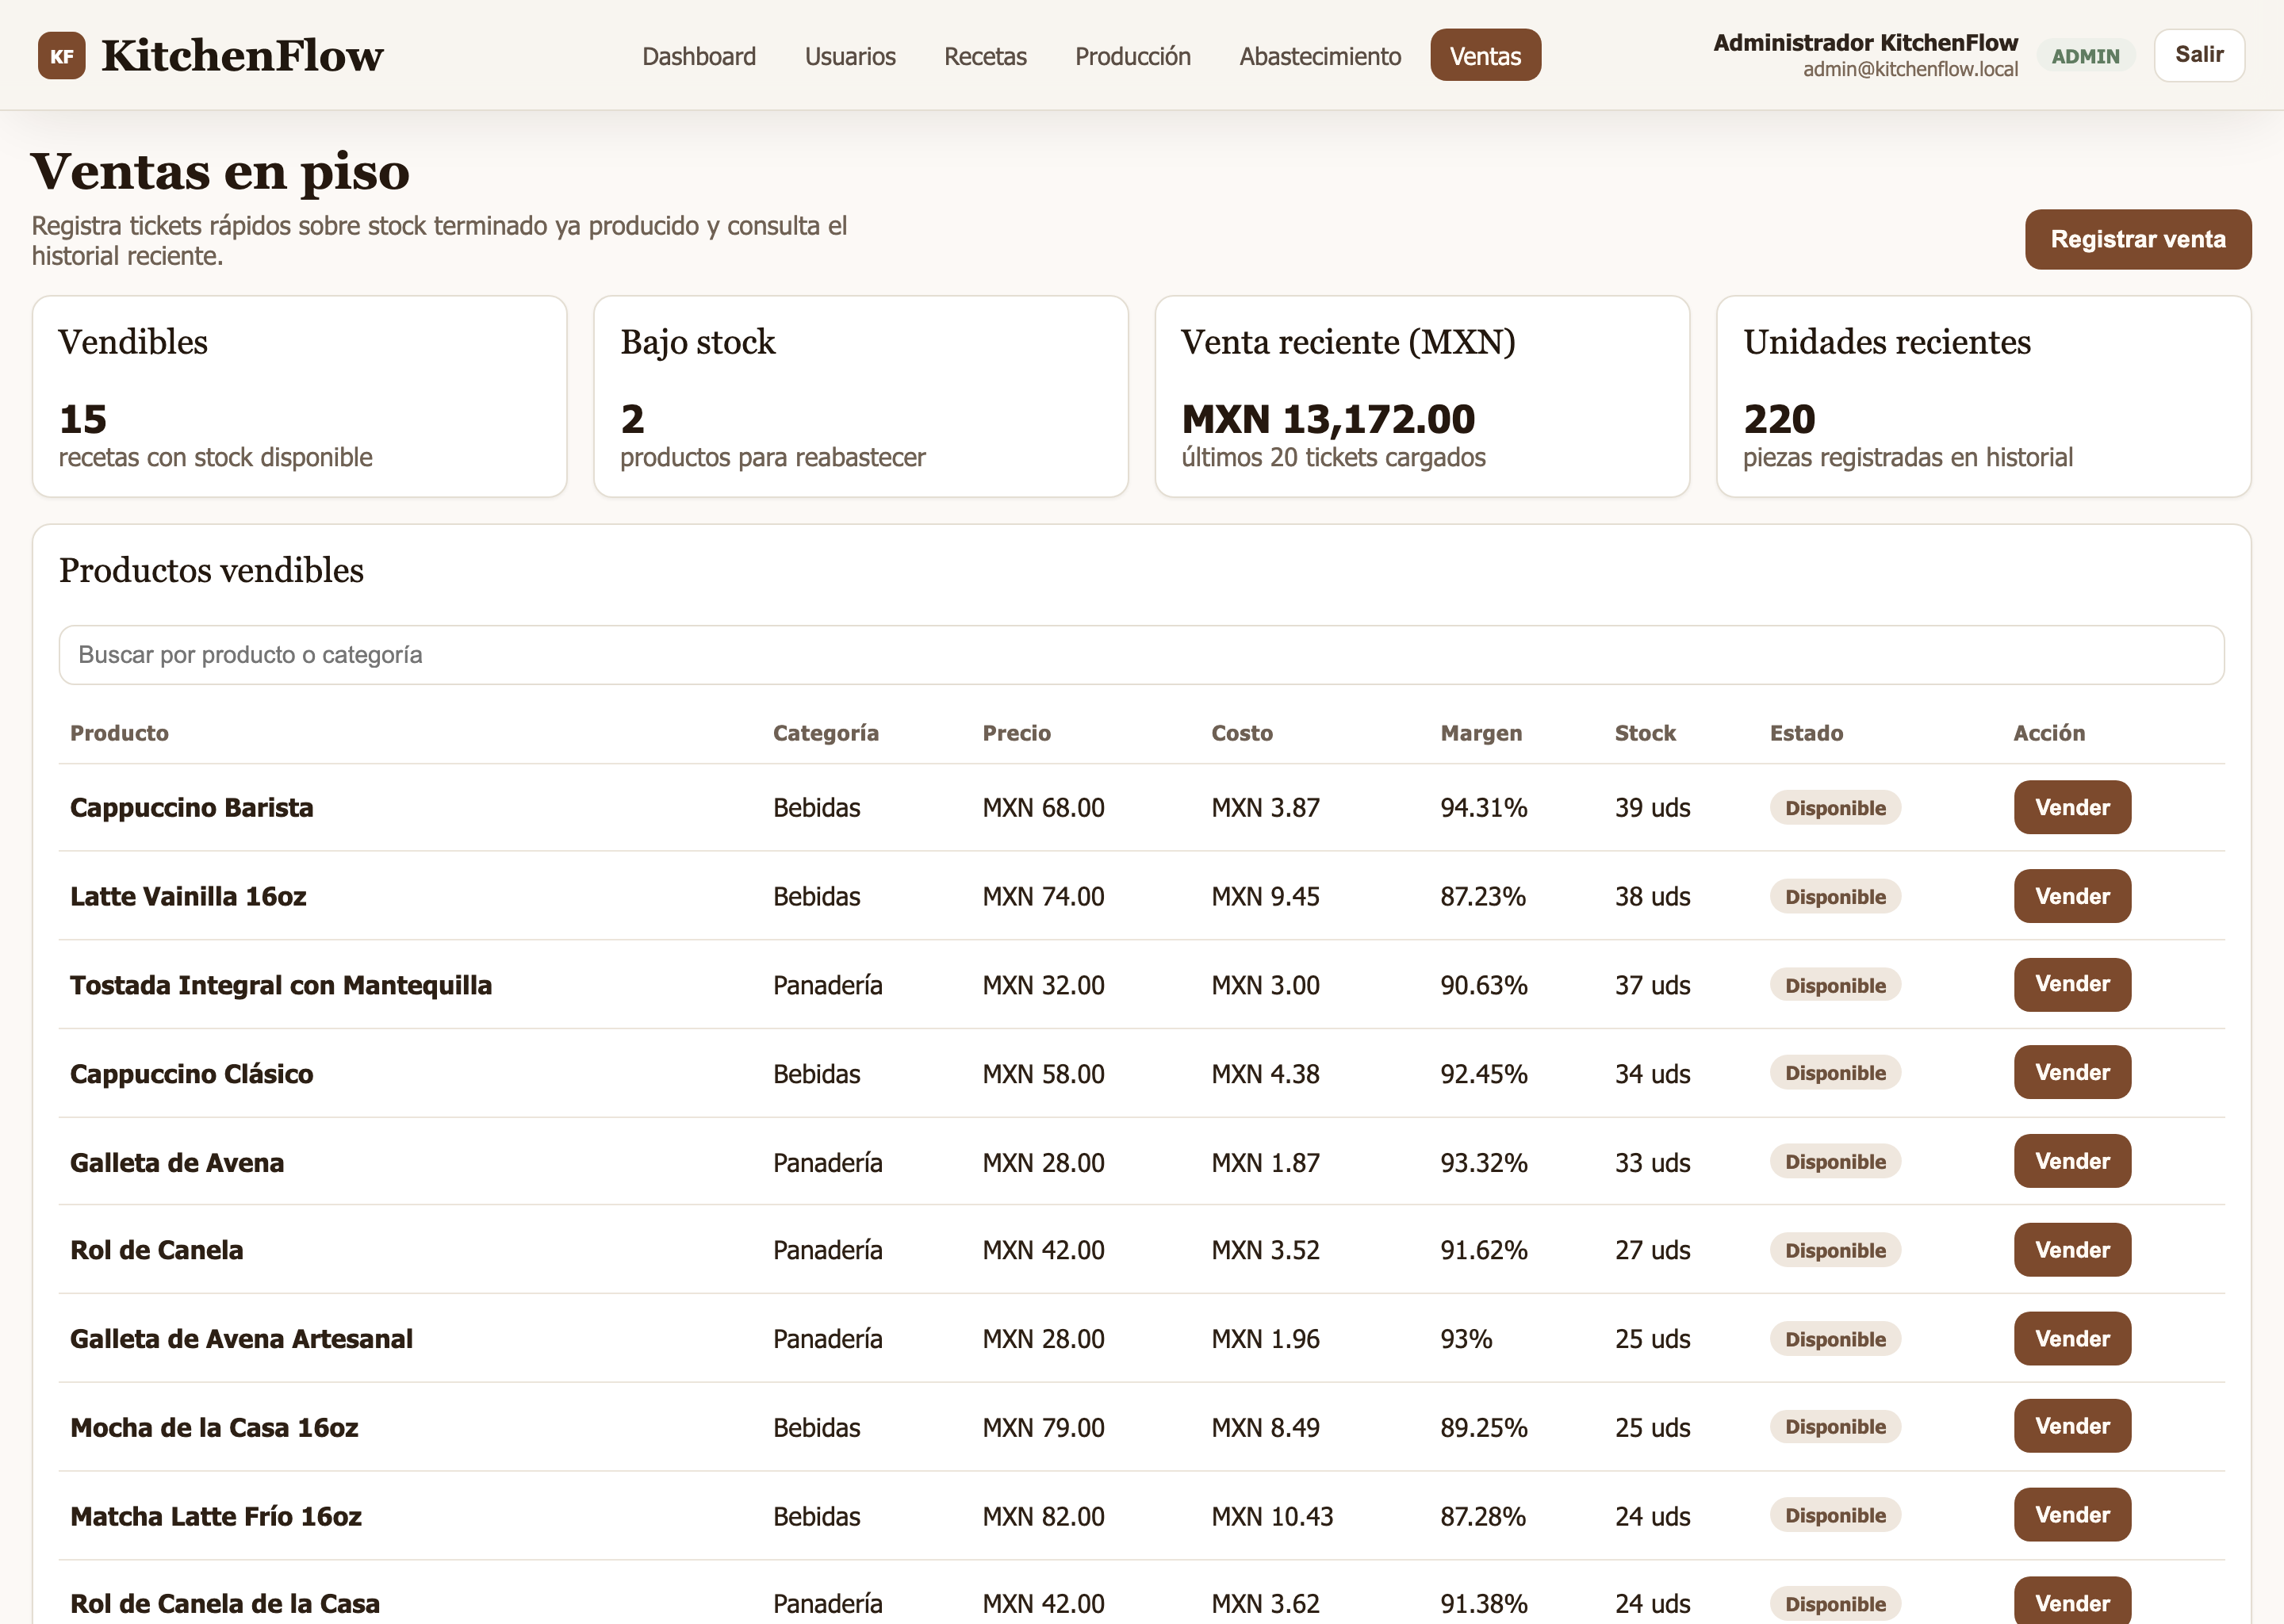
\includegraphics[width=0.92\textwidth,height=0.34\textheight,keepaspectratio]{capturas/ventas.png}
	\caption{Pantalla de ventas en piso con productos vendibles, stock disponible, ticket rápido e historial reciente de ventas.}
\end{figure}

\section{Módulos implementados}

\subsection{Autenticación y autorización}
El sistema implementa autenticación con JWT, recuperación de sesión y protección de acceso por rol. Existen tres perfiles operativos:

\begin{itemize}
	\item \textbf{Administrador}: acceso a dashboard, usuarios, abastecimiento, recetas, producción y ventas.
	\item \textbf{Cocina}: acceso a recetas y producción.
	\item \textbf{Piso}: acceso a ventas.
\end{itemize}

\subsection{Abastecimiento}
El módulo de abastecimiento permite registrar insumos, consultar su stock mínimo, revisar historial de compras y registrar recepciones con recálculo de costo promedio ponderado.

\subsection{Recetas y costeo}
Las recetas almacenan insumos, cantidades, costo total, precio de venta y margen. El sistema permite evaluar rentabilidad por receta y mantener el stock terminado asociado al producto.

\subsection{Producción}
La producción fue implementada como un flujo con estados operativos:
\begin{itemize}
	\item \texttt{PENDING}
	\item \texttt{IN\_PROGRESS}
	\item \texttt{COMPLETED}
	\item \texttt{CANCELLED}
\end{itemize}

Durante este flujo se apartan insumos, se valida disponibilidad, se registra consumo real y se calcula el costo de merma por lote.

\subsection{Ventas}
El módulo de ventas registra tickets reales, descuenta stock terminado y conserva snapshots de precio, costo y margen por línea de venta.

\subsection{Dashboard}
El dashboard presenta indicadores reales de operación: ventas, margen bruto, compras, merma, productos más vendidos, alertas de inventario y actividad reciente de producción.

\subsection{Gestión de usuarios}
Se implementó una pantalla administrativa para alta, edición de rol, activación/desactivación y restablecimiento de contraseña. Con esto se cubre la responsabilidad operativa del rol administrador definida en la propuesta.

\section{Elementos no críticos ajustados por alcance}
No se identifican ausencias funcionales críticas de primer orden respecto al alcance aprobado del proyecto. Los ajustes pendientes o simplificados se concentran en decisiones de alcance controlado:

\begin{itemize}
	\item la \textbf{conversión genérica de unidades} no fue desarrollada como motor separado, ya que el sistema trabaja con un catálogo normalizado de captura;
	\item el manejo de \textbf{mermas} no vive en una pantalla exclusiva, pero la información sí se registra y se usa en producción y dashboard;
	\item la arquitectura final no reproduce literalmente el stack declarado en la propuesta, pero sí resuelve los mismos objetivos funcionales.
\end{itemize}

\section{Conclusión}
La implementación final de \textbf{KitchenFlow} conserva el propósito central de la propuesta: controlar insumos, costear recetas, transformar materia prima en producto terminado, registrar ventas y exponer indicadores de rentabilidad para la toma de decisiones.

Las diferencias detectadas frente al documento original se explican principalmente por:
\begin{itemize}
	\item decisiones de arquitectura más adecuadas al stack real del repositorio;
	\item mejoras de flujo de trabajo en la interfaz;
	\item integración de ciertas funciones en módulos más operativos.
\end{itemize}

En términos de entrega, el proyecto puede considerarse \textbf{funcionalmente implementado en su núcleo principal}. Las variaciones observadas son, en su mayoría, ajustes razonables de implementación y no omisiones graves del objetivo del sistema.

\end{document}
